
% Default to the notebook output style

    


% Inherit from the specified cell style.




    
\documentclass[11pt]{article}

    
    
    \usepackage[T1]{fontenc}
    % Nicer default font (+ math font) than Computer Modern for most use cases
    \usepackage{mathpazo}

    % Basic figure setup, for now with no caption control since it's done
    % automatically by Pandoc (which extracts ![](path) syntax from Markdown).
    \usepackage{graphicx}
    % We will generate all images so they have a width \maxwidth. This means
    % that they will get their normal width if they fit onto the page, but
    % are scaled down if they would overflow the margins.
    \makeatletter
    \def\maxwidth{\ifdim\Gin@nat@width>\linewidth\linewidth
    \else\Gin@nat@width\fi}
    \makeatother
    \let\Oldincludegraphics\includegraphics
    % Set max figure width to be 80% of text width, for now hardcoded.
    \renewcommand{\includegraphics}[1]{\Oldincludegraphics[width=.8\maxwidth]{#1}}
    % Ensure that by default, figures have no caption (until we provide a
    % proper Figure object with a Caption API and a way to capture that
    % in the conversion process - todo).
    \usepackage{caption}
    \DeclareCaptionLabelFormat{nolabel}{}
    \captionsetup{labelformat=nolabel}

    \usepackage{adjustbox} % Used to constrain images to a maximum size 
    \usepackage{xcolor} % Allow colors to be defined
    \usepackage{enumerate} % Needed for markdown enumerations to work
    \usepackage{geometry} % Used to adjust the document margins
    \usepackage{amsmath} % Equations
    \usepackage{amssymb} % Equations
    \usepackage{textcomp} % defines textquotesingle
    % Hack from http://tex.stackexchange.com/a/47451/13684:
    \AtBeginDocument{%
        \def\PYZsq{\textquotesingle}% Upright quotes in Pygmentized code
    }
    \usepackage{upquote} % Upright quotes for verbatim code
    \usepackage{eurosym} % defines \euro
    \usepackage[mathletters]{ucs} % Extended unicode (utf-8) support
    \usepackage[utf8x]{inputenc} % Allow utf-8 characters in the tex document
    \usepackage{fancyvrb} % verbatim replacement that allows latex
    \usepackage{grffile} % extends the file name processing of package graphics 
                         % to support a larger range 
    % The hyperref package gives us a pdf with properly built
    % internal navigation ('pdf bookmarks' for the table of contents,
    % internal cross-reference links, web links for URLs, etc.)
    \usepackage{hyperref}
    \usepackage{longtable} % longtable support required by pandoc >1.10
    \usepackage{booktabs}  % table support for pandoc > 1.12.2
    \usepackage[inline]{enumitem} % IRkernel/repr support (it uses the enumerate* environment)
    \usepackage[normalem]{ulem} % ulem is needed to support strikethroughs (\sout)
                                % normalem makes italics be italics, not underlines
    

    
    
    % Colors for the hyperref package
    \definecolor{urlcolor}{rgb}{0,.145,.698}
    \definecolor{linkcolor}{rgb}{.71,0.21,0.01}
    \definecolor{citecolor}{rgb}{.12,.54,.11}

    % ANSI colors
    \definecolor{ansi-black}{HTML}{3E424D}
    \definecolor{ansi-black-intense}{HTML}{282C36}
    \definecolor{ansi-red}{HTML}{E75C58}
    \definecolor{ansi-red-intense}{HTML}{B22B31}
    \definecolor{ansi-green}{HTML}{00A250}
    \definecolor{ansi-green-intense}{HTML}{007427}
    \definecolor{ansi-yellow}{HTML}{DDB62B}
    \definecolor{ansi-yellow-intense}{HTML}{B27D12}
    \definecolor{ansi-blue}{HTML}{208FFB}
    \definecolor{ansi-blue-intense}{HTML}{0065CA}
    \definecolor{ansi-magenta}{HTML}{D160C4}
    \definecolor{ansi-magenta-intense}{HTML}{A03196}
    \definecolor{ansi-cyan}{HTML}{60C6C8}
    \definecolor{ansi-cyan-intense}{HTML}{258F8F}
    \definecolor{ansi-white}{HTML}{C5C1B4}
    \definecolor{ansi-white-intense}{HTML}{A1A6B2}

    % commands and environments needed by pandoc snippets
    % extracted from the output of `pandoc -s`
    \providecommand{\tightlist}{%
      \setlength{\itemsep}{0pt}\setlength{\parskip}{0pt}}
    \DefineVerbatimEnvironment{Highlighting}{Verbatim}{commandchars=\\\{\}}
    % Add ',fontsize=\small' for more characters per line
    \newenvironment{Shaded}{}{}
    \newcommand{\KeywordTok}[1]{\textcolor[rgb]{0.00,0.44,0.13}{\textbf{{#1}}}}
    \newcommand{\DataTypeTok}[1]{\textcolor[rgb]{0.56,0.13,0.00}{{#1}}}
    \newcommand{\DecValTok}[1]{\textcolor[rgb]{0.25,0.63,0.44}{{#1}}}
    \newcommand{\BaseNTok}[1]{\textcolor[rgb]{0.25,0.63,0.44}{{#1}}}
    \newcommand{\FloatTok}[1]{\textcolor[rgb]{0.25,0.63,0.44}{{#1}}}
    \newcommand{\CharTok}[1]{\textcolor[rgb]{0.25,0.44,0.63}{{#1}}}
    \newcommand{\StringTok}[1]{\textcolor[rgb]{0.25,0.44,0.63}{{#1}}}
    \newcommand{\CommentTok}[1]{\textcolor[rgb]{0.38,0.63,0.69}{\textit{{#1}}}}
    \newcommand{\OtherTok}[1]{\textcolor[rgb]{0.00,0.44,0.13}{{#1}}}
    \newcommand{\AlertTok}[1]{\textcolor[rgb]{1.00,0.00,0.00}{\textbf{{#1}}}}
    \newcommand{\FunctionTok}[1]{\textcolor[rgb]{0.02,0.16,0.49}{{#1}}}
    \newcommand{\RegionMarkerTok}[1]{{#1}}
    \newcommand{\ErrorTok}[1]{\textcolor[rgb]{1.00,0.00,0.00}{\textbf{{#1}}}}
    \newcommand{\NormalTok}[1]{{#1}}
    
    % Additional commands for more recent versions of Pandoc
    \newcommand{\ConstantTok}[1]{\textcolor[rgb]{0.53,0.00,0.00}{{#1}}}
    \newcommand{\SpecialCharTok}[1]{\textcolor[rgb]{0.25,0.44,0.63}{{#1}}}
    \newcommand{\VerbatimStringTok}[1]{\textcolor[rgb]{0.25,0.44,0.63}{{#1}}}
    \newcommand{\SpecialStringTok}[1]{\textcolor[rgb]{0.73,0.40,0.53}{{#1}}}
    \newcommand{\ImportTok}[1]{{#1}}
    \newcommand{\DocumentationTok}[1]{\textcolor[rgb]{0.73,0.13,0.13}{\textit{{#1}}}}
    \newcommand{\AnnotationTok}[1]{\textcolor[rgb]{0.38,0.63,0.69}{\textbf{\textit{{#1}}}}}
    \newcommand{\CommentVarTok}[1]{\textcolor[rgb]{0.38,0.63,0.69}{\textbf{\textit{{#1}}}}}
    \newcommand{\VariableTok}[1]{\textcolor[rgb]{0.10,0.09,0.49}{{#1}}}
    \newcommand{\ControlFlowTok}[1]{\textcolor[rgb]{0.00,0.44,0.13}{\textbf{{#1}}}}
    \newcommand{\OperatorTok}[1]{\textcolor[rgb]{0.40,0.40,0.40}{{#1}}}
    \newcommand{\BuiltInTok}[1]{{#1}}
    \newcommand{\ExtensionTok}[1]{{#1}}
    \newcommand{\PreprocessorTok}[1]{\textcolor[rgb]{0.74,0.48,0.00}{{#1}}}
    \newcommand{\AttributeTok}[1]{\textcolor[rgb]{0.49,0.56,0.16}{{#1}}}
    \newcommand{\InformationTok}[1]{\textcolor[rgb]{0.38,0.63,0.69}{\textbf{\textit{{#1}}}}}
    \newcommand{\WarningTok}[1]{\textcolor[rgb]{0.38,0.63,0.69}{\textbf{\textit{{#1}}}}}
    
    
    % Define a nice break command that doesn't care if a line doesn't already
    % exist.
    \def\br{\hspace*{\fill} \\* }
    % Math Jax compatability definitions
    \def\gt{>}
    \def\lt{<}
    % Document parameters
    \title{lecture\_11}
    
    
    

    % Pygments definitions
    
\makeatletter
\def\PY@reset{\let\PY@it=\relax \let\PY@bf=\relax%
    \let\PY@ul=\relax \let\PY@tc=\relax%
    \let\PY@bc=\relax \let\PY@ff=\relax}
\def\PY@tok#1{\csname PY@tok@#1\endcsname}
\def\PY@toks#1+{\ifx\relax#1\empty\else%
    \PY@tok{#1}\expandafter\PY@toks\fi}
\def\PY@do#1{\PY@bc{\PY@tc{\PY@ul{%
    \PY@it{\PY@bf{\PY@ff{#1}}}}}}}
\def\PY#1#2{\PY@reset\PY@toks#1+\relax+\PY@do{#2}}

\expandafter\def\csname PY@tok@gd\endcsname{\def\PY@tc##1{\textcolor[rgb]{0.63,0.00,0.00}{##1}}}
\expandafter\def\csname PY@tok@gu\endcsname{\let\PY@bf=\textbf\def\PY@tc##1{\textcolor[rgb]{0.50,0.00,0.50}{##1}}}
\expandafter\def\csname PY@tok@gt\endcsname{\def\PY@tc##1{\textcolor[rgb]{0.00,0.27,0.87}{##1}}}
\expandafter\def\csname PY@tok@gs\endcsname{\let\PY@bf=\textbf}
\expandafter\def\csname PY@tok@gr\endcsname{\def\PY@tc##1{\textcolor[rgb]{1.00,0.00,0.00}{##1}}}
\expandafter\def\csname PY@tok@cm\endcsname{\let\PY@it=\textit\def\PY@tc##1{\textcolor[rgb]{0.25,0.50,0.50}{##1}}}
\expandafter\def\csname PY@tok@vg\endcsname{\def\PY@tc##1{\textcolor[rgb]{0.10,0.09,0.49}{##1}}}
\expandafter\def\csname PY@tok@vi\endcsname{\def\PY@tc##1{\textcolor[rgb]{0.10,0.09,0.49}{##1}}}
\expandafter\def\csname PY@tok@mh\endcsname{\def\PY@tc##1{\textcolor[rgb]{0.40,0.40,0.40}{##1}}}
\expandafter\def\csname PY@tok@cs\endcsname{\let\PY@it=\textit\def\PY@tc##1{\textcolor[rgb]{0.25,0.50,0.50}{##1}}}
\expandafter\def\csname PY@tok@ge\endcsname{\let\PY@it=\textit}
\expandafter\def\csname PY@tok@vc\endcsname{\def\PY@tc##1{\textcolor[rgb]{0.10,0.09,0.49}{##1}}}
\expandafter\def\csname PY@tok@il\endcsname{\def\PY@tc##1{\textcolor[rgb]{0.40,0.40,0.40}{##1}}}
\expandafter\def\csname PY@tok@go\endcsname{\def\PY@tc##1{\textcolor[rgb]{0.53,0.53,0.53}{##1}}}
\expandafter\def\csname PY@tok@cp\endcsname{\def\PY@tc##1{\textcolor[rgb]{0.74,0.48,0.00}{##1}}}
\expandafter\def\csname PY@tok@gi\endcsname{\def\PY@tc##1{\textcolor[rgb]{0.00,0.63,0.00}{##1}}}
\expandafter\def\csname PY@tok@gh\endcsname{\let\PY@bf=\textbf\def\PY@tc##1{\textcolor[rgb]{0.00,0.00,0.50}{##1}}}
\expandafter\def\csname PY@tok@ni\endcsname{\let\PY@bf=\textbf\def\PY@tc##1{\textcolor[rgb]{0.60,0.60,0.60}{##1}}}
\expandafter\def\csname PY@tok@nl\endcsname{\def\PY@tc##1{\textcolor[rgb]{0.63,0.63,0.00}{##1}}}
\expandafter\def\csname PY@tok@nn\endcsname{\let\PY@bf=\textbf\def\PY@tc##1{\textcolor[rgb]{0.00,0.00,1.00}{##1}}}
\expandafter\def\csname PY@tok@no\endcsname{\def\PY@tc##1{\textcolor[rgb]{0.53,0.00,0.00}{##1}}}
\expandafter\def\csname PY@tok@na\endcsname{\def\PY@tc##1{\textcolor[rgb]{0.49,0.56,0.16}{##1}}}
\expandafter\def\csname PY@tok@nb\endcsname{\def\PY@tc##1{\textcolor[rgb]{0.00,0.50,0.00}{##1}}}
\expandafter\def\csname PY@tok@nc\endcsname{\let\PY@bf=\textbf\def\PY@tc##1{\textcolor[rgb]{0.00,0.00,1.00}{##1}}}
\expandafter\def\csname PY@tok@nd\endcsname{\def\PY@tc##1{\textcolor[rgb]{0.67,0.13,1.00}{##1}}}
\expandafter\def\csname PY@tok@ne\endcsname{\let\PY@bf=\textbf\def\PY@tc##1{\textcolor[rgb]{0.82,0.25,0.23}{##1}}}
\expandafter\def\csname PY@tok@nf\endcsname{\def\PY@tc##1{\textcolor[rgb]{0.00,0.00,1.00}{##1}}}
\expandafter\def\csname PY@tok@si\endcsname{\let\PY@bf=\textbf\def\PY@tc##1{\textcolor[rgb]{0.73,0.40,0.53}{##1}}}
\expandafter\def\csname PY@tok@s2\endcsname{\def\PY@tc##1{\textcolor[rgb]{0.73,0.13,0.13}{##1}}}
\expandafter\def\csname PY@tok@nt\endcsname{\let\PY@bf=\textbf\def\PY@tc##1{\textcolor[rgb]{0.00,0.50,0.00}{##1}}}
\expandafter\def\csname PY@tok@nv\endcsname{\def\PY@tc##1{\textcolor[rgb]{0.10,0.09,0.49}{##1}}}
\expandafter\def\csname PY@tok@s1\endcsname{\def\PY@tc##1{\textcolor[rgb]{0.73,0.13,0.13}{##1}}}
\expandafter\def\csname PY@tok@ch\endcsname{\let\PY@it=\textit\def\PY@tc##1{\textcolor[rgb]{0.25,0.50,0.50}{##1}}}
\expandafter\def\csname PY@tok@m\endcsname{\def\PY@tc##1{\textcolor[rgb]{0.40,0.40,0.40}{##1}}}
\expandafter\def\csname PY@tok@gp\endcsname{\let\PY@bf=\textbf\def\PY@tc##1{\textcolor[rgb]{0.00,0.00,0.50}{##1}}}
\expandafter\def\csname PY@tok@sh\endcsname{\def\PY@tc##1{\textcolor[rgb]{0.73,0.13,0.13}{##1}}}
\expandafter\def\csname PY@tok@ow\endcsname{\let\PY@bf=\textbf\def\PY@tc##1{\textcolor[rgb]{0.67,0.13,1.00}{##1}}}
\expandafter\def\csname PY@tok@sx\endcsname{\def\PY@tc##1{\textcolor[rgb]{0.00,0.50,0.00}{##1}}}
\expandafter\def\csname PY@tok@bp\endcsname{\def\PY@tc##1{\textcolor[rgb]{0.00,0.50,0.00}{##1}}}
\expandafter\def\csname PY@tok@c1\endcsname{\let\PY@it=\textit\def\PY@tc##1{\textcolor[rgb]{0.25,0.50,0.50}{##1}}}
\expandafter\def\csname PY@tok@o\endcsname{\def\PY@tc##1{\textcolor[rgb]{0.40,0.40,0.40}{##1}}}
\expandafter\def\csname PY@tok@kc\endcsname{\let\PY@bf=\textbf\def\PY@tc##1{\textcolor[rgb]{0.00,0.50,0.00}{##1}}}
\expandafter\def\csname PY@tok@c\endcsname{\let\PY@it=\textit\def\PY@tc##1{\textcolor[rgb]{0.25,0.50,0.50}{##1}}}
\expandafter\def\csname PY@tok@mf\endcsname{\def\PY@tc##1{\textcolor[rgb]{0.40,0.40,0.40}{##1}}}
\expandafter\def\csname PY@tok@err\endcsname{\def\PY@bc##1{\setlength{\fboxsep}{0pt}\fcolorbox[rgb]{1.00,0.00,0.00}{1,1,1}{\strut ##1}}}
\expandafter\def\csname PY@tok@mb\endcsname{\def\PY@tc##1{\textcolor[rgb]{0.40,0.40,0.40}{##1}}}
\expandafter\def\csname PY@tok@ss\endcsname{\def\PY@tc##1{\textcolor[rgb]{0.10,0.09,0.49}{##1}}}
\expandafter\def\csname PY@tok@sr\endcsname{\def\PY@tc##1{\textcolor[rgb]{0.73,0.40,0.53}{##1}}}
\expandafter\def\csname PY@tok@mo\endcsname{\def\PY@tc##1{\textcolor[rgb]{0.40,0.40,0.40}{##1}}}
\expandafter\def\csname PY@tok@kd\endcsname{\let\PY@bf=\textbf\def\PY@tc##1{\textcolor[rgb]{0.00,0.50,0.00}{##1}}}
\expandafter\def\csname PY@tok@mi\endcsname{\def\PY@tc##1{\textcolor[rgb]{0.40,0.40,0.40}{##1}}}
\expandafter\def\csname PY@tok@kn\endcsname{\let\PY@bf=\textbf\def\PY@tc##1{\textcolor[rgb]{0.00,0.50,0.00}{##1}}}
\expandafter\def\csname PY@tok@cpf\endcsname{\let\PY@it=\textit\def\PY@tc##1{\textcolor[rgb]{0.25,0.50,0.50}{##1}}}
\expandafter\def\csname PY@tok@kr\endcsname{\let\PY@bf=\textbf\def\PY@tc##1{\textcolor[rgb]{0.00,0.50,0.00}{##1}}}
\expandafter\def\csname PY@tok@s\endcsname{\def\PY@tc##1{\textcolor[rgb]{0.73,0.13,0.13}{##1}}}
\expandafter\def\csname PY@tok@kp\endcsname{\def\PY@tc##1{\textcolor[rgb]{0.00,0.50,0.00}{##1}}}
\expandafter\def\csname PY@tok@w\endcsname{\def\PY@tc##1{\textcolor[rgb]{0.73,0.73,0.73}{##1}}}
\expandafter\def\csname PY@tok@kt\endcsname{\def\PY@tc##1{\textcolor[rgb]{0.69,0.00,0.25}{##1}}}
\expandafter\def\csname PY@tok@sc\endcsname{\def\PY@tc##1{\textcolor[rgb]{0.73,0.13,0.13}{##1}}}
\expandafter\def\csname PY@tok@sb\endcsname{\def\PY@tc##1{\textcolor[rgb]{0.73,0.13,0.13}{##1}}}
\expandafter\def\csname PY@tok@k\endcsname{\let\PY@bf=\textbf\def\PY@tc##1{\textcolor[rgb]{0.00,0.50,0.00}{##1}}}
\expandafter\def\csname PY@tok@se\endcsname{\let\PY@bf=\textbf\def\PY@tc##1{\textcolor[rgb]{0.73,0.40,0.13}{##1}}}
\expandafter\def\csname PY@tok@sd\endcsname{\let\PY@it=\textit\def\PY@tc##1{\textcolor[rgb]{0.73,0.13,0.13}{##1}}}

\def\PYZbs{\char`\\}
\def\PYZus{\char`\_}
\def\PYZob{\char`\{}
\def\PYZcb{\char`\}}
\def\PYZca{\char`\^}
\def\PYZam{\char`\&}
\def\PYZlt{\char`\<}
\def\PYZgt{\char`\>}
\def\PYZsh{\char`\#}
\def\PYZpc{\char`\%}
\def\PYZdl{\char`\$}
\def\PYZhy{\char`\-}
\def\PYZsq{\char`\'}
\def\PYZdq{\char`\"}
\def\PYZti{\char`\~}
% for compatibility with earlier versions
\def\PYZat{@}
\def\PYZlb{[}
\def\PYZrb{]}
\makeatother


    % Exact colors from NB
    \definecolor{incolor}{rgb}{0.0, 0.0, 0.5}
    \definecolor{outcolor}{rgb}{0.545, 0.0, 0.0}



    
    % Prevent overflowing lines due to hard-to-break entities
    \sloppy 
    % Setup hyperref package
    \hypersetup{
      breaklinks=true,  % so long urls are correctly broken across lines
      colorlinks=true,
      urlcolor=urlcolor,
      linkcolor=linkcolor,
      citecolor=citecolor,
      }
    % Slightly bigger margins than the latex defaults
    
    \geometry{verbose,tmargin=1in,bmargin=1in,lmargin=1in,rmargin=1in}
    
    

    \begin{document}
    
    
    \maketitle
    
    

    
    \begin{Verbatim}[commandchars=\\\{\}]
{\color{incolor}In [{\color{incolor}1}]:} \PY{c}{\PYZpc{}plot \PYZhy{}\PYZhy{}format svg}
\end{Verbatim}

    \begin{Verbatim}[commandchars=\\\{\}]
{\color{incolor}In [{\color{incolor}2}]:} \PY{n}{setdefaults}
\end{Verbatim}

    \subsection{My question from last
class}\label{my-question-from-last-class}

\(A=\left[ \begin{array}{ccc} 10 & 2 & 1 \\ 0 & 1 & 1 \\ 0 & 0 & 10\end{array} \right]\)

\begin{figure}[htbp]
\centering
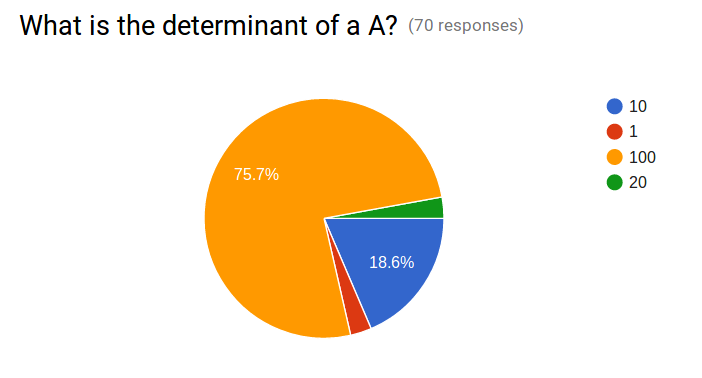
\includegraphics{det_A.png}
\caption{responses to determinant of A}
\end{figure}

\subsection{Your questions from last
class}\label{your-questions-from-last-class}

\begin{enumerate}
\def\labelenumi{\arabic{enumi}.}
\item
  Need more linear algebra review

  -We will keep doing Linear Algebra, try the practice problems in
  'linear\_algebra'
\item
  How do I do HW3?

  -demo today
\item
  For hw4 is the spring constant (K) suppose to be given?

  -yes, its 30 N/m
\item
  Deapool or Joker?
\end{enumerate}

\subsection{Midterm preference}\label{midterm-preference}

\begin{figure}[htbp]
\centering
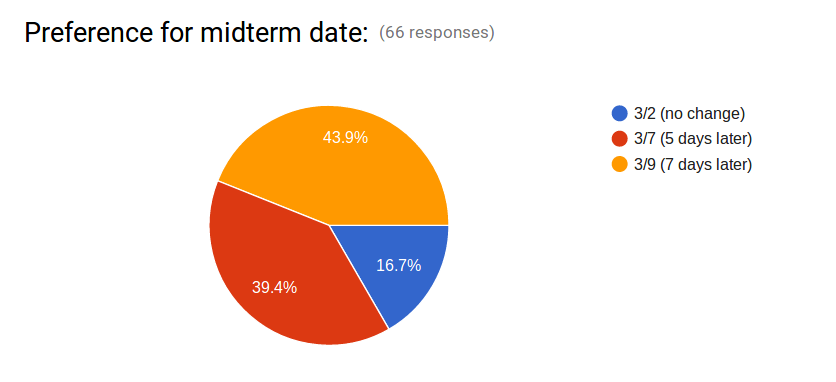
\includegraphics{midterm_date.png}
\caption{responses to midterm date}
\end{figure}

\subsubsection{Midterm Questions}\label{midterm-questions}

\begin{enumerate}
\def\labelenumi{\arabic{enumi}.}
\item
  Notes allowed

  -no
\item
  Will there be a review/study sheet

  -yes
\end{enumerate}

    \section{LU Decomposition}\label{lu-decomposition}

\subsubsection{efficient storage of matrices for
solutions}\label{efficient-storage-of-matrices-for-solutions}

Considering the same solution set:

\(y=Ax\)

Assume that we can perform Gauss elimination and achieve this formula:

\(Ux=d\)

Where, \(U\) is an upper triangular matrix that we derived from Gauss
elimination and \(d\) is the set of dependent variables after Gauss
elimination.

Assume there is a lower triangular matrix, \(L\), with ones on the
diagonal and same dimensions of \(U\) and the following is true:

\(L(Ux-d)=Ax-y=0\)

Now, \(Ax=LUx\), so \(A=LU\), and \(y=Ld\).

\(2x_{1}+x_{2}=1\)

\(x_{1}+3x_{2}=1\)

\(\left[ \begin{array}{cc} 2 & 1 \\ 1 & 3 \end{array} \right] \left[\begin{array}{c} x_{1} \\ x_{2} \end{array}\right]= \left[\begin{array}{c} 1 \\ 1\end{array}\right]\)

f21=0.5

A(2,1)=1-1 = 0

A(2,2)=3-0.5=2.5

y(2)=1-0.5=0.5

\(L(Ux-d)= \left[ \begin{array}{cc} 1 & 0 \\ 0.5 & 1 \end{array} \right] \left(\left[ \begin{array}{cc} 2 & 1 \\ 0 & 2.5 \end{array} \right] \left[\begin{array}{c} x_{1} \\ x_{2} \end{array}\right]- \left[\begin{array}{c} 1 \\ 0.5\end{array}\right]\right)=0\)

    \begin{Verbatim}[commandchars=\\\{\}]
{\color{incolor}In [{\color{incolor}3}]:} \PY{n}{A}\PY{p}{=}\PY{p}{[}\PY{l+m+mi}{2}\PY{p}{,}\PY{l+m+mi}{1}\PY{p}{;}\PY{l+m+mi}{1}\PY{p}{,}\PY{l+m+mi}{3}\PY{p}{]}
        \PY{n}{L}\PY{p}{=}\PY{p}{[}\PY{l+m+mi}{1}\PY{p}{,}\PY{l+m+mi}{0}\PY{p}{;}\PY{l+m+mf}{0.5}\PY{p}{,}\PY{l+m+mi}{1}\PY{p}{]}
        \PY{n}{U}\PY{p}{=}\PY{p}{[}\PY{l+m+mi}{2}\PY{p}{,}\PY{l+m+mi}{1}\PY{p}{;}\PY{l+m+mi}{0}\PY{p}{,}\PY{l+m+mf}{2.5}\PY{p}{]}
        \PY{n}{L}\PY{o}{*}\PY{n}{U}
        
        \PY{n}{d}\PY{p}{=}\PY{p}{[}\PY{l+m+mi}{1}\PY{p}{;}\PY{l+m+mf}{0.5}\PY{p}{]}
        \PY{n}{y}\PY{p}{=}\PY{n}{L}\PY{o}{*}\PY{n}{d}
\end{Verbatim}

    \begin{Verbatim}[commandchars=\\\{\}]
A =

   2   1
   1   3

L =

   1.00000   0.00000
   0.50000   1.00000

U =

   2.00000   1.00000
   0.00000   2.50000

ans =

   2   1
   1   3

d =

   1.00000
   0.50000

y =

   1
   1


    \end{Verbatim}

    \begin{Verbatim}[commandchars=\\\{\}]
{\color{incolor}In [{\color{incolor}5}]:} \PY{c}{\PYZpc{} what is the determinant of L, U and A?}
        
        \PY{n+nb}{det}\PY{p}{(}\PY{n}{A}\PY{p}{)}
        \PY{n+nb}{det}\PY{p}{(}\PY{n}{L}\PY{p}{)}
        \PY{n+nb}{det}\PY{p}{(}\PY{n}{U}\PY{p}{)}
        \PY{n+nb}{det}\PY{p}{(}\PY{n}{L}\PY{p}{)}\PY{o}{*}\PY{n+nb}{det}\PY{p}{(}\PY{n}{U}\PY{p}{)}
        \PY{n+nb}{det}\PY{p}{(}\PY{n}{L}\PY{o}{*}\PY{n}{U}\PY{p}{)}
\end{Verbatim}

    \begin{Verbatim}[commandchars=\\\{\}]
ans =  5.0000
ans =  1
ans =  5
ans =  5
ans =  5.0000

    \end{Verbatim}

    \subsection{Pivoting for LU
factorization}\label{pivoting-for-lu-factorization}

LU factorization uses the same method as Gauss elimination so it is also
necessary to perform partial pivoting when creating the lower and upper
triangular matrices.

Matlab and Octave use pivoting in the command

\texttt{{[}L,U,P{]}=lu(A)}

    \begin{Verbatim}[commandchars=\\\{\}]
{\color{incolor}In [{\color{incolor}4}]:} \PY{n}{help} \PY{n+nb}{lu}
\end{Verbatim}

    \begin{Verbatim}[commandchars=\\\{\}]
'lu' is a built-in function from the file libinterp/corefcn/lu.cc

 -- Built-in Function: [L, U] = lu (A)
 -- Built-in Function: [L, U, P] = lu (A)
 -- Built-in Function: [L, U, P, Q] = lu (S)
 -- Built-in Function: [L, U, P, Q, R] = lu (S)
 -- Built-in Function: [{\ldots}] = lu (S, THRES)
 -- Built-in Function: Y = lu ({\ldots})
 -- Built-in Function: [{\ldots}] = lu ({\ldots}, "vector")
     Compute the LU decomposition of A.

     If A is full subroutines from LAPACK are used and if A is sparse
     then UMFPACK is used.

     The result is returned in a permuted form, according to the
     optional return value P.  For example, given the matrix 'a = [1, 2;
     3, 4]',

          [l, u, p] = lu (A)

     returns

          l =

            1.00000  0.00000
            0.33333  1.00000

          u =

            3.00000  4.00000
            0.00000  0.66667

          p =

            0  1
            1  0

     The matrix is not required to be square.

     When called with two or three output arguments and a spare input
     matrix, 'lu' does not attempt to perform sparsity preserving column
     permutations.  Called with a fourth output argument, the sparsity
     preserving column transformation Q is returned, such that 'P * A *
     Q = L * U'.

     Called with a fifth output argument and a sparse input matrix, 'lu'
     attempts to use a scaling factor R on the input matrix such that 'P
     * (R \textbackslash{} A) * Q = L * U'.  This typically leads to a sparser and more
     stable factorization.

     An additional input argument THRES, that defines the pivoting
     threshold can be given.  THRES can be a scalar, in which case it
     defines the UMFPACK pivoting tolerance for both symmetric and
     unsymmetric cases.  If THRES is a 2-element vector, then the first
     element defines the pivoting tolerance for the unsymmetric UMFPACK
     pivoting strategy and the second for the symmetric strategy.  By
     default, the values defined by 'spparms' are used ([0.1, 0.001]).

     Given the string argument "vector", 'lu' returns the values of P
     and Q as vector values, such that for full matrix, 'A (P,:) = L *
     U', and 'R(P,:) * A (:, Q) = L * U'.

     With two output arguments, returns the permuted forms of the upper
     and lower triangular matrices, such that 'A = L * U'.  With one
     output argument Y, then the matrix returned by the LAPACK routines
     is returned.  If the input matrix is sparse then the matrix L is
     embedded into U to give a return value similar to the full case.
     For both full and sparse matrices, 'lu' loses the permutation
     information.

     See also: luupdate, ilu, chol, hess, qr, qz, schur, svd.

Additional help for built-in functions and operators is
available in the online version of the manual.  Use the command
'doc <topic>' to search the manual index.

Help and information about Octave is also available on the WWW
at http://www.octave.org and via the help@octave.org
mailing list.

    \end{Verbatim}

    \begin{Verbatim}[commandchars=\\\{\}]
{\color{incolor}In [{\color{incolor}9}]:} \PY{c}{\PYZpc{} time LU solution vs backslash}
        \PY{n}{t\PYZus{}lu}\PY{p}{=}\PY{n+nb}{zeros}\PY{p}{(}\PY{l+m+mi}{100}\PY{p}{,}\PY{l+m+mi}{1}\PY{p}{)}\PY{p}{;}
        \PY{n}{t\PYZus{}bs}\PY{p}{=}\PY{n+nb}{zeros}\PY{p}{(}\PY{l+m+mi}{100}\PY{p}{,}\PY{l+m+mi}{1}\PY{p}{)}\PY{p}{;}
        \PY{k}{for} \PY{n}{N}\PY{p}{=}\PY{l+m+mi}{1}\PY{p}{:}\PY{l+m+mi}{100}
            \PY{n}{A}\PY{p}{=}\PY{n+nb}{rand}\PY{p}{(}\PY{n}{N}\PY{p}{,}\PY{n}{N}\PY{p}{)}\PY{p}{;}
            \PY{n}{y}\PY{p}{=}\PY{n+nb}{rand}\PY{p}{(}\PY{n}{N}\PY{p}{,}\PY{l+m+mi}{1}\PY{p}{)}\PY{p}{;}
            \PY{p}{[}\PY{n}{L}\PY{p}{,}\PY{n}{U}\PY{p}{,}\PY{n}{P}\PY{p}{]}\PY{p}{=}\PY{n+nb}{lu}\PY{p}{(}\PY{n}{A}\PY{p}{)}\PY{p}{;}
        
            \PY{n+nb}{tic}\PY{p}{;} \PY{n}{d}\PY{p}{=}\PY{n+nb}{inv}\PY{p}{(}\PY{n}{L}\PY{p}{)}\PY{o}{*}\PY{n}{y}\PY{p}{;} \PY{n}{x}\PY{p}{=}\PY{n+nb}{inv}\PY{p}{(}\PY{n}{U}\PY{p}{)}\PY{o}{*}\PY{n}{d}\PY{p}{;} \PY{n}{t\PYZus{}lu}\PY{p}{(}\PY{n}{N}\PY{p}{)}\PY{p}{=}\PY{n+nb}{toc}\PY{p}{;}
        
            \PY{n+nb}{tic}\PY{p}{;} \PY{n}{x}\PY{p}{=}\PY{n+nb}{inv}\PY{p}{(}\PY{n}{A}\PY{p}{)}\PY{o}{*}\PY{n}{y}\PY{p}{;} \PY{n}{t\PYZus{}bs}\PY{p}{(}\PY{n}{N}\PY{p}{)}\PY{p}{=}\PY{n+nb}{toc}\PY{p}{;}
        \PY{k}{end}
        \PY{n+nb}{plot}\PY{p}{(}\PY{p}{[}\PY{l+m+mi}{1}\PY{p}{:}\PY{l+m+mi}{100}\PY{p}{]}\PY{p}{,}\PY{n}{t\PYZus{}lu}\PY{p}{,}\PY{p}{[}\PY{l+m+mi}{1}\PY{p}{:}\PY{l+m+mi}{100}\PY{p}{]}\PY{p}{,}\PY{n}{t\PYZus{}bs}\PY{p}{)} 
        \PY{n+nb}{legend}\PY{p}{(}\PY{l+s}{\PYZsq{}}\PY{l+s}{LU decomp\PYZsq{}}\PY{p}{,}\PY{l+s}{\PYZsq{}}\PY{l+s}{Octave \PYZbs{}\PYZbs{}\PYZsq{}}\PY{p}{)}
\end{Verbatim}

    \begin{center}
    \adjustimage{max size={0.9\linewidth}{0.9\paperheight}}{lecture_11_files/lecture_11_8_0.pdf}
    \end{center}
    { \hspace*{\fill} \\}
    
    Consider the problem again from the intro to Linear Algebra, 4 masses
are connected in series to 4 springs with K=10 N/m. What are the final
positions of the masses?

\begin{figure}[htbp]
\centering
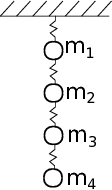
\includegraphics{../lecture_09/mass_springs.png}
\caption{Springs-masses}
\end{figure}

The masses haves the following amounts, 1, 2, 3, and 4 kg for masses
1-4. Using a FBD for each mass:

\(m_{1}g+k(x_{2}-x_{1})-kx_{1}=0\)

\(m_{2}g+k(x_{3}-x_{2})-k(x_{2}-x_{1})=0\)

\(m_{3}g+k(x_{4}-x_{3})-k(x_{3}-x_{2})=0\)

\(m_{4}g-k(x_{4}-x_{3})=0\)

in matrix form:

\(\left[ \begin{array}{cccc} 2k & -k & 0 & 0 \\ -k & 2k & -k & 0 \\ 0 & -k & 2k & -k \\ 0 & 0 & -k & k \end{array} \right] \left[ \begin{array}{c} x_{1} \\ x_{2} \\ x_{3} \\ x_{4} \end{array} \right]= \left[ \begin{array}{c} m_{1}g \\ m_{2}g \\ m_{3}g \\ m_{4}g \end{array} \right]\)

    \begin{Verbatim}[commandchars=\\\{\}]
{\color{incolor}In [{\color{incolor}10}]:} \PY{n}{k}\PY{p}{=}\PY{l+m+mi}{10}\PY{p}{;} \PY{c}{\PYZpc{} N/m}
         \PY{n}{m1}\PY{p}{=}\PY{l+m+mi}{1}\PY{p}{;} \PY{c}{\PYZpc{} kg}
         \PY{n}{m2}\PY{p}{=}\PY{l+m+mi}{2}\PY{p}{;}
         \PY{n}{m3}\PY{p}{=}\PY{l+m+mi}{3}\PY{p}{;}
         \PY{n}{m4}\PY{p}{=}\PY{l+m+mi}{4}\PY{p}{;}
         \PY{n}{g}\PY{p}{=}\PY{l+m+mf}{9.81}\PY{p}{;} \PY{c}{\PYZpc{} m/s\PYZca{}2}
         \PY{n}{K}\PY{p}{=}\PY{p}{[}\PY{l+m+mi}{2}\PY{o}{*}\PY{n}{k} \PY{o}{\PYZhy{}}\PY{n}{k} \PY{l+m+mi}{0} \PY{l+m+mi}{0}\PY{p}{;} \PY{o}{\PYZhy{}}\PY{n}{k} \PY{l+m+mi}{2}\PY{o}{*}\PY{n}{k} \PY{o}{\PYZhy{}}\PY{n}{k} \PY{l+m+mi}{0}\PY{p}{;} \PY{l+m+mi}{0} \PY{o}{\PYZhy{}}\PY{n}{k} \PY{l+m+mi}{2}\PY{o}{*}\PY{n}{k} \PY{o}{\PYZhy{}}\PY{n}{k}\PY{p}{;} \PY{l+m+mi}{0} \PY{l+m+mi}{0} \PY{o}{\PYZhy{}}\PY{n}{k} \PY{n}{k}\PY{p}{]}
         \PY{n}{y}\PY{p}{=}\PY{p}{[}\PY{n}{m1}\PY{o}{*}\PY{n}{g}\PY{p}{;}\PY{n}{m2}\PY{o}{*}\PY{n}{g}\PY{p}{;}\PY{n}{m3}\PY{o}{*}\PY{n}{g}\PY{p}{;}\PY{n}{m4}\PY{o}{*}\PY{n}{g}\PY{p}{]}
\end{Verbatim}

    \begin{Verbatim}[commandchars=\\\{\}]
K =

   20  -10    0    0
  -10   20  -10    0
    0  -10   20  -10
    0    0  -10   10

y =

    9.8100
   19.6200
   29.4300
   39.2400


    \end{Verbatim}

    This matrix, K, is symmetric.

\texttt{K(i,j)==K(j,i)}

Now we can use,

\subsection{Cholesky Factorization}\label{cholesky-factorization}

We can decompose the matrix, K into two matrices, \(U\) and \(U^{T}\),
where

\(K=U^{T}U\)

each of the components of U can be calculated with the following
equations:

\(u_{ii}=\sqrt{a_{ii}-\sum_{k=1}^{i-1}u_{ki}^{2}}\)

\(u_{ij}=\frac{a_{ij}-\sum_{k=1}^{i-1}u_{ki}u_{kj}}{u_{ii}}\)

so for K

    \begin{Verbatim}[commandchars=\\\{\}]
{\color{incolor}In [{\color{incolor}11}]:} \PY{n}{K}
\end{Verbatim}

    \begin{Verbatim}[commandchars=\\\{\}]
K =

   20  -10    0    0
  -10   20  -10    0
    0  -10   20  -10
    0    0  -10   10


    \end{Verbatim}

    \begin{Verbatim}[commandchars=\\\{\}]
{\color{incolor}In [{\color{incolor}12}]:} \PY{n}{u11}\PY{p}{=}\PY{n+nb}{sqrt}\PY{p}{(}\PY{n}{K}\PY{p}{(}\PY{l+m+mi}{1}\PY{p}{,}\PY{l+m+mi}{1}\PY{p}{)}\PY{p}{)}
         \PY{n}{u12}\PY{p}{=}\PY{p}{(}\PY{n}{K}\PY{p}{(}\PY{l+m+mi}{1}\PY{p}{,}\PY{l+m+mi}{2}\PY{p}{)}\PY{p}{)}\PY{o}{/}\PY{n}{u11}
         \PY{n}{u13}\PY{p}{=}\PY{p}{(}\PY{n}{K}\PY{p}{(}\PY{l+m+mi}{1}\PY{p}{,}\PY{l+m+mi}{3}\PY{p}{)}\PY{p}{)}\PY{o}{/}\PY{n}{u11}
         \PY{n}{u14}\PY{p}{=}\PY{p}{(}\PY{n}{K}\PY{p}{(}\PY{l+m+mi}{1}\PY{p}{,}\PY{l+m+mi}{4}\PY{p}{)}\PY{p}{)}\PY{o}{/}\PY{n}{u11}
         \PY{n}{u22}\PY{p}{=}\PY{n+nb}{sqrt}\PY{p}{(}\PY{n}{K}\PY{p}{(}\PY{l+m+mi}{2}\PY{p}{,}\PY{l+m+mi}{2}\PY{p}{)}\PY{o}{\PYZhy{}}\PY{n}{u12}\PYZca{}\PY{l+m+mi}{2}\PY{p}{)}
         \PY{n}{u23}\PY{p}{=}\PY{p}{(}\PY{n}{K}\PY{p}{(}\PY{l+m+mi}{2}\PY{p}{,}\PY{l+m+mi}{3}\PY{p}{)}\PY{o}{\PYZhy{}}\PY{n}{u12}\PY{o}{*}\PY{n}{u13}\PY{p}{)}\PY{o}{/}\PY{n}{u22}
         \PY{n}{u24}\PY{p}{=}\PY{p}{(}\PY{n}{K}\PY{p}{(}\PY{l+m+mi}{2}\PY{p}{,}\PY{l+m+mi}{4}\PY{p}{)}\PY{o}{\PYZhy{}}\PY{n}{u12}\PY{o}{*}\PY{n}{u14}\PY{p}{)}\PY{o}{/}\PY{n}{u22}
         \PY{n}{u33}\PY{p}{=}\PY{n+nb}{sqrt}\PY{p}{(}\PY{n}{K}\PY{p}{(}\PY{l+m+mi}{3}\PY{p}{,}\PY{l+m+mi}{3}\PY{p}{)}\PY{o}{\PYZhy{}}\PY{n}{u13}\PYZca{}\PY{l+m+mi}{2}\PY{o}{\PYZhy{}}\PY{n}{u23}\PYZca{}\PY{l+m+mi}{2}\PY{p}{)}
         \PY{n}{u34}\PY{p}{=}\PY{p}{(}\PY{n}{K}\PY{p}{(}\PY{l+m+mi}{3}\PY{p}{,}\PY{l+m+mi}{4}\PY{p}{)}\PY{o}{\PYZhy{}}\PY{n}{u13}\PY{o}{*}\PY{n}{u14}\PY{o}{\PYZhy{}}\PY{n}{u23}\PY{o}{*}\PY{n}{u24}\PY{p}{)}\PY{o}{/}\PY{n}{u33}
         \PY{n}{u44}\PY{p}{=}\PY{n+nb}{sqrt}\PY{p}{(}\PY{n}{K}\PY{p}{(}\PY{l+m+mi}{4}\PY{p}{,}\PY{l+m+mi}{4}\PY{p}{)}\PY{o}{\PYZhy{}}\PY{n}{u14}\PYZca{}\PY{l+m+mi}{2}\PY{o}{\PYZhy{}}\PY{n}{u24}\PYZca{}\PY{l+m+mi}{2}\PY{o}{\PYZhy{}}\PY{n}{u34}\PYZca{}\PY{l+m+mi}{2}\PY{p}{)}
         \PY{n}{U}\PY{p}{=}\PY{p}{[}\PY{n}{u11}\PY{p}{,}\PY{n}{u12}\PY{p}{,}\PY{n}{u13}\PY{p}{,}\PY{n}{u14}\PY{p}{;}\PY{l+m+mi}{0}\PY{p}{,}\PY{n}{u22}\PY{p}{,}\PY{n}{u23}\PY{p}{,}\PY{n}{u24}\PY{p}{;}\PY{l+m+mi}{0}\PY{p}{,}\PY{l+m+mi}{0}\PY{p}{,}\PY{n}{u33}\PY{p}{,}\PY{n}{u34}\PY{p}{;}\PY{l+m+mi}{0}\PY{p}{,}\PY{l+m+mi}{0}\PY{p}{,}\PY{l+m+mi}{0}\PY{p}{,}\PY{n}{u44}\PY{p}{]}
\end{Verbatim}

    \begin{Verbatim}[commandchars=\\\{\}]
u11 =  4.4721
u12 = -2.2361
u13 = 0
u14 = 0
u22 =  3.8730
u23 = -2.5820
u24 = 0
u33 =  3.6515
u34 = -2.7386
u44 =  1.5811
U =

   4.47214  -2.23607   0.00000   0.00000
   0.00000   3.87298  -2.58199   0.00000
   0.00000   0.00000   3.65148  -2.73861
   0.00000   0.00000   0.00000   1.58114


    \end{Verbatim}

    \begin{Verbatim}[commandchars=\\\{\}]
{\color{incolor}In [{\color{incolor}17}]:} \PY{p}{(}\PY{n}{U}\PY{o}{\PYZsq{}}\PY{o}{*}\PY{n}{U}\PY{p}{)}\PY{o}{\PYZsq{}}\PY{o}{==}\PY{n}{U}\PY{o}{\PYZsq{}}\PY{o}{*}\PY{n}{U}
\end{Verbatim}

    \begin{Verbatim}[commandchars=\\\{\}]
ans =

   1   1   1   1
   1   1   1   1
   1   1   1   1
   1   1   1   1


    \end{Verbatim}

    \begin{Verbatim}[commandchars=\\\{\}]
{\color{incolor}In [{\color{incolor}18}]:} \PY{c}{\PYZpc{} time solution for Cholesky vs backslash}
         \PY{n}{t\PYZus{}chol}\PY{p}{=}\PY{n+nb}{zeros}\PY{p}{(}\PY{l+m+mi}{1000}\PY{p}{,}\PY{l+m+mi}{1}\PY{p}{)}\PY{p}{;}
         \PY{n}{t\PYZus{}bs}\PY{p}{=}\PY{n+nb}{zeros}\PY{p}{(}\PY{l+m+mi}{1000}\PY{p}{,}\PY{l+m+mi}{1}\PY{p}{)}\PY{p}{;}
         \PY{k}{for} \PY{n}{i}\PY{p}{=}\PY{l+m+mi}{1}\PY{p}{:}\PY{l+m+mi}{1000}
             \PY{n+nb}{tic}\PY{p}{;} \PY{n}{d}\PY{p}{=}\PY{n}{U}\PY{o}{\PYZsq{}}\PY{o}{*}\PY{n}{y}\PY{p}{;} \PY{n}{x}\PY{p}{=}\PY{n}{U}\PY{o}{\PYZbs{}}\PY{n}{d}\PY{p}{;} \PY{n}{t\PYZus{}chol}\PY{p}{(}\PY{n}{i}\PY{p}{)}\PY{p}{=}\PY{n+nb}{toc}\PY{p}{;}
             \PY{n+nb}{tic}\PY{p}{;} \PY{n}{x}\PY{p}{=}\PY{n}{K}\PY{o}{\PYZbs{}}\PY{n}{y}\PY{p}{;} \PY{n}{t\PYZus{}bs}\PY{p}{(}\PY{n}{i}\PY{p}{)}\PY{p}{=}\PY{n+nb}{toc}\PY{p}{;}
         \PY{k}{end}
         \PY{n+nb}{fprintf}\PY{p}{(}\PY{l+s}{\PYZsq{}}\PY{l+s}{average time spent for Cholesky factored solution = \PYZpc{}e+/\PYZhy{}\PYZpc{}e\PYZsq{}}\PY{p}{,}\PY{n+nb}{mean}\PY{p}{(}\PY{n}{t\PYZus{}chol}\PY{p}{)}\PY{p}{,}\PY{n+nb}{std}\PY{p}{(}\PY{n}{t\PYZus{}chol}\PY{p}{)}\PY{p}{)}
         
         \PY{n+nb}{fprintf}\PY{p}{(}\PY{l+s}{\PYZsq{}}\PY{l+s}{average time spent for backslash solution         = \PYZpc{}e+/\PYZhy{}\PYZpc{}e\PYZsq{}}\PY{p}{,}\PY{n+nb}{mean}\PY{p}{(}\PY{n}{t\PYZus{}bs}\PY{p}{)}\PY{p}{,}\PY{n+nb}{std}\PY{p}{(}\PY{n}{t\PYZus{}bs}\PY{p}{)}\PY{p}{)}
\end{Verbatim}

    \begin{Verbatim}[commandchars=\\\{\}]
average time spent for Cholesky factored solution = 1.465964e-05+/-9.806001e-06
average time spent for backslash solution         = 1.555967e-05+/-1.048561e-05

    \end{Verbatim}

    \begin{Verbatim}[commandchars=\\\{\}]
{\color{incolor}In [{\color{incolor} }]:} 
\end{Verbatim}


    % Add a bibliography block to the postdoc
    
    
    
    \end{document}
